%===================================== CHAP 3 =================================

\chapter{Empiric Review}
\section{CASE: The Life Science Building-project}
The project case will examine the construction of the new life science building of the University of Oslo. When finished, the building will reach a cost of approximately 6,8 million Norwegian Kroner (NOK), and cover 66,700 square meters, with this, becoming the most extensive, detached university building in Norway. Construction builder is the Norwegian Directorate of Public Construction and Property Management (Statsbygg). The construction started on the 8 of February 2019 and is expected to finish in 2024, while the project management of this report started in 2017.

The manager, Stasbygg, is a significant organization in the Norwegian construction industry. They are on a state mission, which means that they are to realize the politics decided by the government, achieved in architecture, cultural legacy, spatial planning, and environment. 

Each year, Statsbygg constructs about 100 construction projects. Some are more complex than others. The life science Building is one of the more complex. In addition to the construction of new buildings and projects, Statsbygg managing about 600 properties of these 90 outside of Norway. Examples of properties managed by Statsbygg are embassies, royal properties, colleges, and cultural buildings. 

In regards to complexity, the new life science building has to meet several complex requirements: (1) the environmental: The property is to achieve Excellent in the BREEAM NOR classification of sustainable properties; (2) usability: a group of the final users has given their feedback on what they expect from the final building; and (3) technical requirements: The building is to house several faculties, some requires highly technical labs.

\subsection{Project vision and Strategies}
The construcionn of the new Life Science Building is, in many ways, a prestige project. Defined in the vision:
\begin{quotation}
    \textit{"An even better project"}
\end{quotation}
The project is following in the line of previous two large projects running Lean Construction, with Statsbygg as manager. Starting with the Domus Medica construction concluded in 2013. This project was the first Norwegian group applying Lean. This construction was followed by the raising of the new Bergen Academy of Art and Design (BAAD). During these projects, Lean Construction was a significant part of the project management. The first project suffered substantial scope creep, which made the managers take action, applying Lean Design and Systematic Completion \textit{Systematisk Ferdigstillelse} on the BAAD-project. The moves made gave results, and when finished in 2017, the project was by many considered one the most successful (complex) building-constructions completed in Norway.

Based on the the BAAB-project a the \textit{Lean methodology in design and construction}-book \cite{lean_i_praksis} descibing the experience from the project, was made. With the previous history and recomendations from the book, Stasbygg, as a manager, defined five superior strategies in the upcoming LSB-project: 
\begin{enumerate}
    \item The Contract strategy
    \item The Lean strategy
    \item Stretegy of Systematic completion
    \item Digitalization strategy
    \item Logistics strategy
\end{enumerate}
These strategies affect how the project should run and emphasize the focus of the project managers, hopefully leading to a sustainable and productive project. Following are a brief introduction to the different strategies as a context for the case. An holistic view of the strategies in the project are illustrated in figure \ref{fig:strategy}.

\begin{figure}
    \centering
    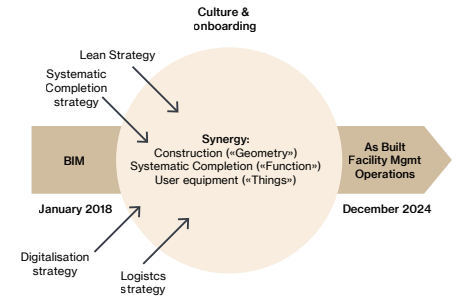
\includegraphics[width=0.8\textwidth]{fig/LVB_strategy.png}
    \caption{A hollistic view of Strategies in the Life Science Building-project.}
    \label{fig:strategy}
\end{figure}

\subsubsection*{The Contract Strategy}
The project has made use of a customized version of the Shared Contract, named by Statsbygg as Shared Contract with Prior Interaction \textit{(Totalentreprise med forutgående Samspill)}. Instead of signing single contracts with each subcontractor, the managers have assembled eight arrangements, each covering different divisions of the project. Hereunder a more Lead Contract type is applied. Figure \ref{fig:project_contracts} displays the eight contract divisions. Responsible for each of the contracts, from management, is either the project manager from construction or technical. 

The motivation for this model is, first, shielding the contractors from some of the risk running this project. The project is, as mentioned, very intricate in construction, as well as in management. Moreover, getting contractors willing to apply on this project, the managers will take much of the risk. Regarding cooperation the projects adds Lead Contracts. The intention of this is cooperation; besides, sharing a contract has the plan of shared responsibility and incentives for collaboration between subcontractors. Even though there is a lead contractor per division, the hope is that the group of subcontractors should feel shared responsibility. Why not have a shared responsibility,and no leading contractor, one may ask? The answer is partly laws and politics, but moreover for simplicity in regards to management; a single point of contact.

\begin{figure}
    \centering
    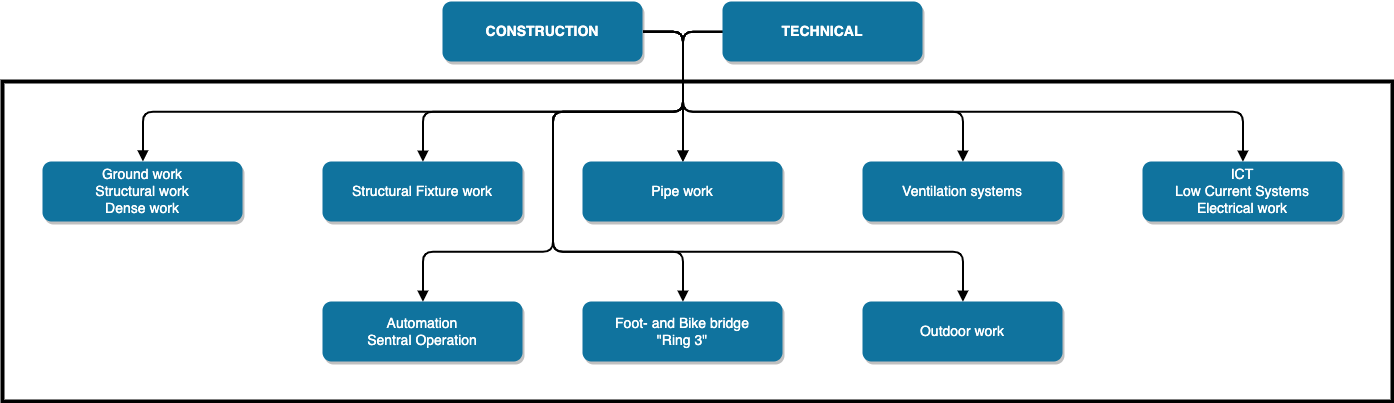
\includegraphics[width=\textwidth]{fig/LVB_contracts.png}
    \caption{Contruction Contracts in the Life Science Building Projects, each managed by either the construction- or technical project manager.}
    \label{fig:project_contracts}
\end{figure}

\subsubsection*{The Lean Strategy}
The Lean Strategy applied in this project is tailor-made from experience from both the Domus Medica- and BAAB-project. Two Lean strategies are applied in the LSB-project: 

\begin{enumerate}
    \item \textbf{Lean Construction:} a method conserning the scheduling
    of tasks and the availability of skills and materials to ensure that the work progresses as smoothly as possiblble during the construction. Keywords are tact, train, and wagon.
    \item \textbf{Lean Design:} a method conserning design management and design coordination. Important is viewing design as a form of product line with BiM as the product.
\end{enumerate}

Different from the traditional design phase described in section \ref{sec:CI_context}, the LSB-project made use of an iterative method, namely the Lean Design-method. In all projects utilizing Lean as their project methodology, this project also iterates over a product. The project, in this context, is the BiM model. The BiM model is the 3-D model of the building. The project makes use of Level of Development (LOD), where each iteration has the intention of getting the BiM model more mature. Also, based on the Contract strategy, the result of this process is not procurement, but the final product ready for implementation - hopefully without bugs. 

Skrive mer om hvorfor dette ble brukt - se side 58 i boka - mye dokumentasjon og endring av req. (tilbakemeldinger) som var en av grunnene til å gå over til Agile.
Legges stor vekt på planlegging av hver fase - Prosesskartet
Nevn Big room - lære av hverandre.

Lean constructing: Forklare kontrollområde, takt, tog, vogn og taktplan
Skrive litt om taktplan og hvordan denne ligner på roadmap. Side 109




\subsubsection*{The Strategy of Systematic Completion}
\subsubsection*{The Digitalization Strategy}
CogitoProject som noe de satser på. 
\subsubsection*{The Logistics Strategy}


\subsection*{Project management in the Life Science Building-project}
To manage a project, this significant, the constructing organization makes use of several different management approaches. One can divide the project management into two levels: (1) process management: The support of the process and how the teams are working together, and in what order; and (2) implementation management or method management: The management of design and implementation of the final product. The organization structure used in the project supports the two levels of project management. The first of the two, process management, are using customized sprint-based process management, adopted from Lean construction. Implementation management using a four-level goal- and tactic-based management.  

The construction project organization structure, as seen in figure \ref{fig:project_structure}. Starting at the top, in charge of the project,is the project director, supported by assisting project director. The board, seen on the right, consists of four managers, each responsible for different strategies of the project. On the left HSE and project support, which is responsible for i.a. communication, economics, progress. Beneath the four divisions in the project, where design is responsible for process and management and paraphernalia for what items should be placed in the final building. Construction and technical are two divisions responsible for 8 contracts.

\begin{figure}
    \centering
    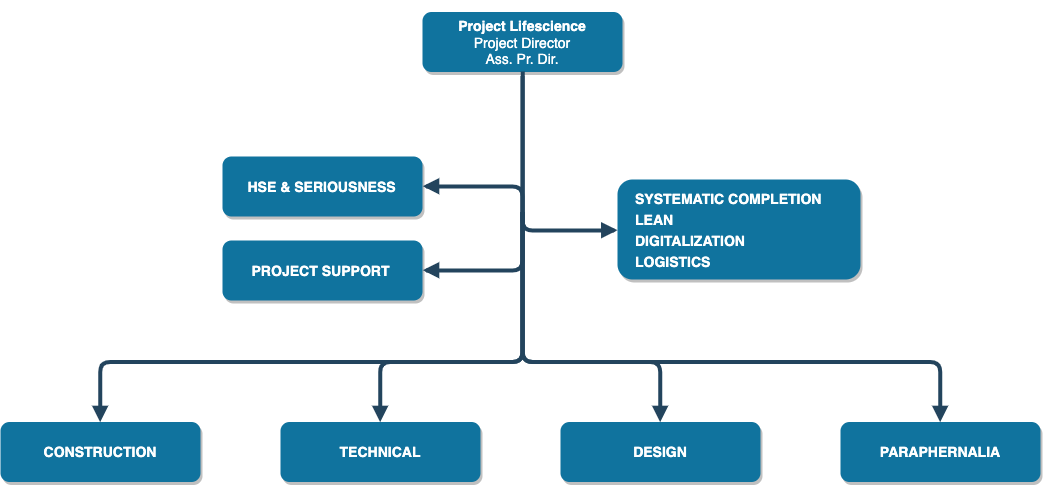
\includegraphics[width=\textwidth]{fig/lvb_diagram.png}
    \caption{Organizational structure in the Life Science Building Project.}
    \label{fig:project_structure}
\end{figure}

Making sure the resulting building is a correct representation of the project vision, process management has developed a customized process. Influenced by agile processes, the method using an iterative process, starting with the vision of the building, ending up with the product; in the form of a finished building. Every iteration has the intention of getting closer to the conclusion, not concluding too early. When every discipline is taken into consideration and satisfied, the project proceeds into the next iteration. Hopefully, this makes for nothing to be redone because no crucial parts are missing. Having these iterations depends on involving disciplines and actors early in the process, which is shown to be demanding.

The implementation management divides into four levels: (1) the Milestones: A significant planned completion of a part of the project, e.g., completion of a floor or start of a new project phase; (2) Key Points: Key Points is less significant, and with a shorter time frame than milestones, but in the same way an indication of completion; (3) Deliveries: Deliveries consists of several Key Points, e.g., finishing a room or design of a floor; and (4) Actions: Actions is everything needed to be done to complete a Delivery. 

\subsubsection{Cooperation in the Life Science Building Project}


\subsubsection{Project management software}

\begin{itemize}
    \item Cogito: Planning and getting information about how much can run in parallel and serial. 
    \item Revit and DRofus
    \item Solibri
    \item Interacso
    \item BIM
\end{itemize}
 
\subsubsection{Project management methods} 
Lean Constructing heavily influences project management in the LSB-project. Some ceremonies applied weekly are Weekly Work Plan (WWP). Every Monday, stakeholders are gathered, checking the status of the project. Identifying progress or mostly lack of it, using Cogito. Deliveries or Key Points are highlighted, and issues been raised. Keeping every stakeholder informed about the status of the project. 


\cleardoublepage